\documentclass{scrreprt}
\usepackage[utf8]{inputenc}
\usepackage[hidelinks]{hyperref}
\usepackage{breakurl}
\usepackage{tabulary}
\usepackage{etoolbox}
\usepackage{graphicx}
%\makeatletter
%\patchcmd{\scr@startchapter}{\if@openright\cleardoublepage\else\clearpage\fi}{}{}{}
%\makeatother

\graphicspath{ {plots/} }

\author{Rick Rongen - 316789 - 2502968}
\title{DS-ML Mini-Project - Diamonds}
\date{\today}

\begin{document}
	\maketitle
	\tableofcontents
	\chapter{Dataset Choses}
		The dataset I'm planning to use is called Diamonds and can be found on Kaggle using the following link: \url{https://www.kaggle.com/shivam2503/diamonds}\par
		
		This dataset describes all kinds of different diamonds with their quality (cut, color, carat and clarity) and size (x, y, z, dept and table). Also it describes the price of the diamond. I would like to use different machine learning techniques to calculate the price of a diamond given one or more of these measurements. Also I would like to be able to do the reverse and see what quality a diamond may be given it's size and price.
		
	\chapter{Example Data}
		In Pandas the cut, color and clarity column will be separated into separate columns or be represented as a number.\par
		Example data:
		\begin{table}[ht]
			\centering
			\caption{Data}
			\label{table-data}
			\begin{tabular}{|l|l|l|l|l|l|l|l|l|l|l|}
				\hline id & carat & cut       & color & clarity & depth & table & price & x    & y    & z    \\ \hline
				1  & 0.23  & Ideal     & E     & SI2     & 61.5  & 55    & 326   & 3.95 & 3.98 & 2.43 \\ \hline
				2  & 0.21  & Premium   & E     & SI1     & 59.8  & 61    & 326   & 3.89 & 3.84 & 2.31 \\ \hline
				3  & 0.23  & Good      & E     & VS1     & 56.9  & 65    & 327   & 4.05 & 4.07 & 2.31 \\ \hline
				4  & 0.29  & Premium   & I     & VS2     & 62.4  & 58    & 334   & 4.2  & 4.23 & 2.63 \\ \hline
				5  & 0.31  & Good      & J     & SI2     & 63.3  & 58    & 335   & 4.34 & 4.35 & 2.75 \\ \hline
				6  & 0.24  & Very Good & J     & VVS2    & 62.8  & 57    & 336   & 3.94 & 3.96 & 2.48 \\ \hline
				7  & 0.24  & Very Good & I     & VVS1    & 62.3  & 57    & 336   & 3.95 & 3.98 & 2.47 \\ \hline
				8  & 0.26  & Very Good & H     & SI1     & 61.9  & 55    & 337   & 4.07 & 4.11 & 2.53 \\ \hline
				9  & 0.22  & Fair      & E     & VS2     & 65.1  & 61    & 337   & 3.87 & 3.78 & 2.49 \\ \hline
				10 & 0.23  & Very Good & H     & VS1     & 59.4  & 61    & 338   & 4    & 4.05 & 2.39 \\ \hline
				11 & 0.3   & Good      & J     & SI1     & 64    & 55    & 339   & 4.25 & 4.28 & 2.73 \\ \hline
				12 & 0.23  & Ideal     & J     & VS1     & 62.8  & 56    & 340   & 3.93 & 3.9  & 2.46 \\ \hline
				13 & 0.22  & Premium   & F     & SI1     & 60.4  & 61    & 342   & 3.88 & 3.84 & 2.33 \\ \hline
				14 & 0.31  & Ideal     & J     & SI2     & 62.2  & 54    & 344   & 4.35 & 4.37 & 2.71 \\ \hline
			\end{tabular}			
		\end{table}
	
		\section{Table Description}
		\begin{tabulary}{\linewidth}{lL}
			carat & Carat weight of the diamond \\\hline
			cut & The cut quality of the diamond. Quality in increasing order Fair, Good, Very Good, Premium, Ideal \\\hline
			color & Color of the diamond, with D being the best and J the worst \\\hline
			clarity & How obvious inclusions are within the diamond:(in order from best to worst, FL = flawless, I3= level 3 inclusions) FL,IF, VVS1, VVS2, VS1, VS2, SI1, SI2, I1, I2, I3 \\\hline
			depth & Total depth percentage = z / mean(x, y) = 2 * z / (x + y) \\\hline
			table & Width of top of diamond relative to widest point  \\\hline
			price & The price of the diamond \\\hline
			x & Length mm \\\hline
			y & Width mm \\\hline
			z & Depth mm \\\hline
		\end{tabulary}
	\chapter{Real World}
	Source: \url{www.info-diamond.com/polished/calculate-diamond-prices.html}\par
	\vspace{2em}
	In the real world a char named the Rapaport chard is commonly used to calculate the price of a diamond. This chart is distributed by the Rapaport organization and costs around 50 USD per chart. These charts are created using the supply and demand statistics from around the world.\par
	A short description of how to calculate the price:
	\begin{enumerate}
		\item Select the correct chart given the shape and carat of the diamond.
		\item Locate the multiplier on the chart using it's color(vertical) and clarity(horizontal).
		\item Multiply the multiplier by the carat of the diamond and then by a 100 to get the price in USD.
	\end{enumerate}
	\chapter{Exploration}
		\begin{figure}[h]
			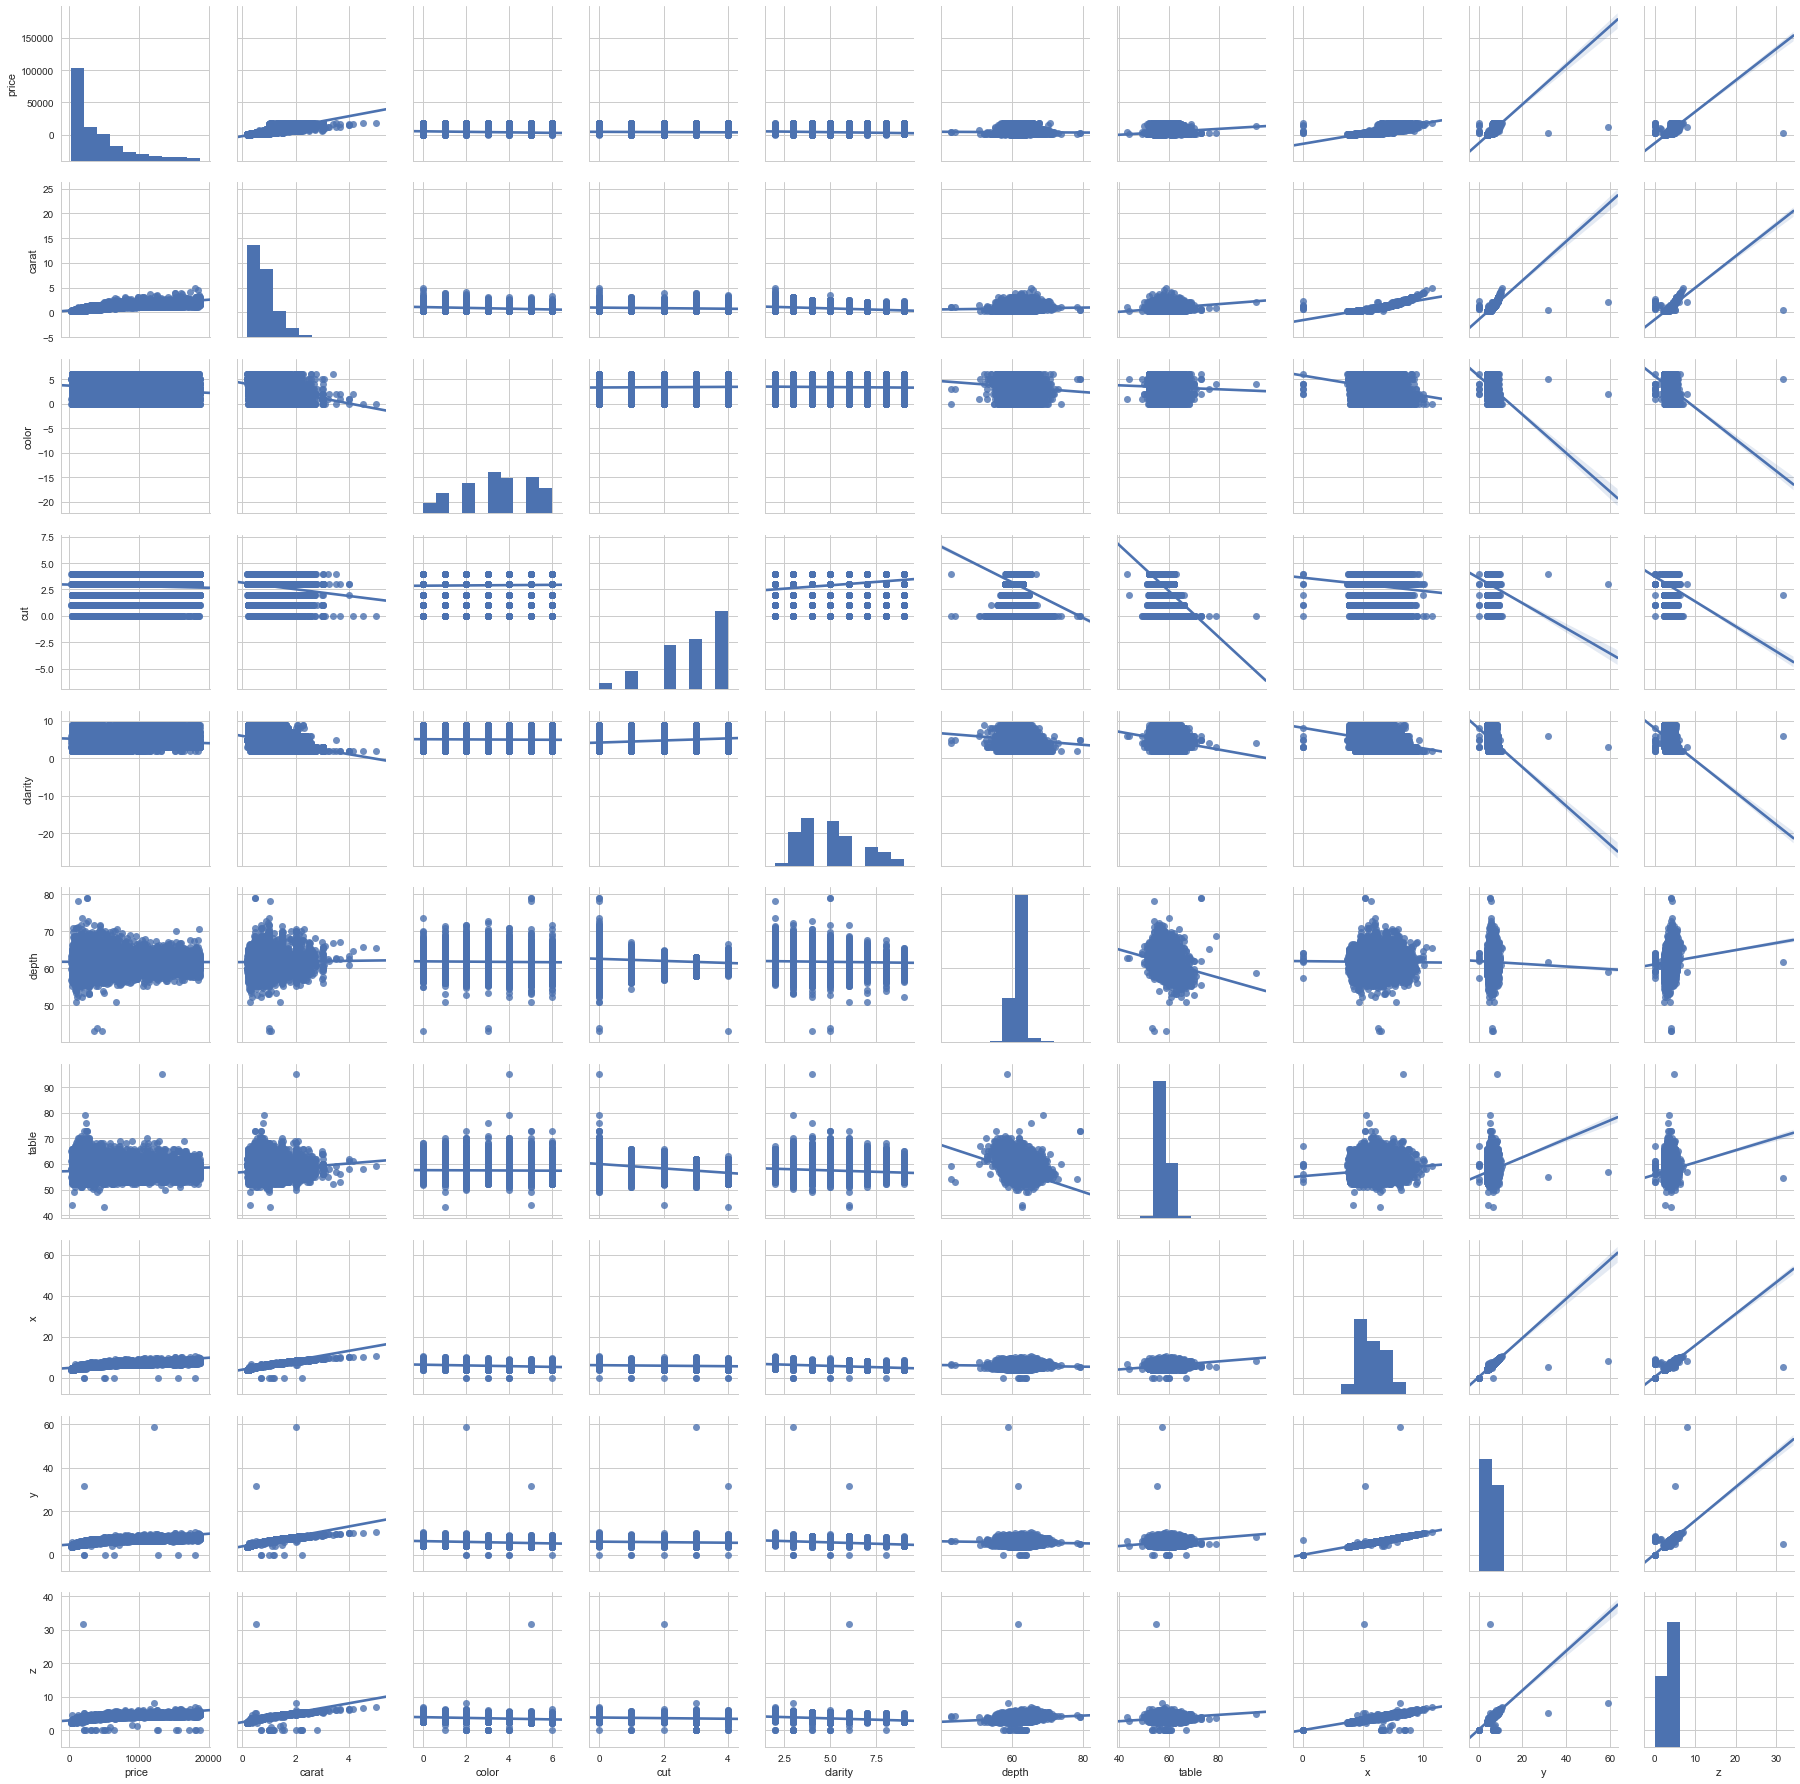
\includegraphics[width=\linewidth]{pairplot}
			\caption{Pairplot all features}
			\label{fig:pairplot}
			\centering
		\end{figure}
		I have plotted all features against each other in \autoref{fig:pairplot}. What I am interested in is the first row and/or the first column, these both relate to the price of the diamonds. In this plot I also executed a regression on all the features to detect any relations.\par
		You can see that the X, Y, Z, table and carat columns have a clear influence on the price. As these values increase, the price also increases. It is strange that the color and clarity do not seem to relate to the price, since they are used in the official price calculation.\par
		
		\begin{figure}[h]
			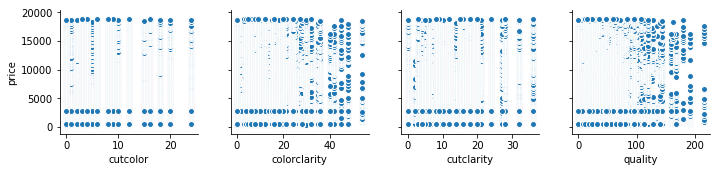
\includegraphics[width=\linewidth]{cut-color-clarity-combi}
			\caption{Combination of Cut, Color and Clarity to price}
			\label{fig:ccc-price}
			\centering
		\end{figure}
		In \autoref{fig:ccc-price} I combined the cut, color and clarity in different ways and compared them to the price. Unfortunately there seems to still not be any evidence to correlation. While I did expect to see some correlation.
		
	\chapter{Learning}
		\section{Hypothesis}
			Using the columns carat, cut, color, clarity, depth, table, x, y and z I can calculate the price of the diamond using one or more machine learning methods.\par
		\section{Execution}
			I have tried 3 different algorithms on the dataset, because I found that these best fit the original price determination. These are Decision Trees, Random Forest and Neural Networks. \par
			I have used GridSearch to find the best parameters for the Decision Tree, but the Random Forest wouldn't even finish the grid search, so I used the same parameters for it. The parameters for the Neural Network where found by trial and error. I used Keras for the Neural Network because it has great customizability.\par
			\subsection{Decison Tree and Random Forest}
				The Decision Tree and the Random Forest have been trained and tested using a KFold split with a K of 5. This helps to reduce over-fitting because each row of data is used for both training and testing but not simultaneously.\par
				The accuracy score for these two algorithms are calculated using the \texttt{r2\_score} of \texttt{sklearn}.\par
			\newpage
			\subsection{Neural Network}
				The Neural Network score is calculated using the \texttt{mean\_squared\_error} function and plotted using the \texttt{live\_loss\_plot} module provided by the Intel workshop. It is optimized using the \texttt{nadam} function. I used this function because after some research on the Keras documentation website I found it was the best fitted function for my usecase. After testing it among some other functions it was clear that this one performed the best. Afterwards the network is also scored using the \texttt{r2\_score} function of sklearn.\par
				\vspace{1em}
				The Neural Network is structured as follows.
				\begin{enumerate}
					\item Dense layer.
						\subitem Nodes: 2*Input
						\subitem Activation: Relu
					\item Dense layer:
						\subitem Nodes: Same as input
						\subitem Activation: Relu
					\item Dense layer:
						\subitem Nodes: 1
						\subitem Activation: Linear
						\subitem Output node
				\end{enumerate}
	\chapter{Findings}
		I found that to some extend the machine learning algorithms are able to predict the price of the diamonds. But often they are a bit off, and sometimes even by a lot. Using the table provided by Rapport seems to be a better option.\par
		The Decision Tree and the Random Forest score with 88\% and 92\% respectively. This already quite accurate, but still have a significant delta in a lot of the cases.\par
		\vspace{1em}
		The Neural Network performed pretty good. Using the \texttt{r2\_score} it got an accuracy of approximately 97.5\%. This seems like a really good score. But when I look at the predictions I see deltas that are quite significant in my opinion.\par
		\vspace{1em}
		When combining the three methods, the score actually deceases from the Neural Network. It becomes 96.8\%. However when looking at the percentiles, a different story is told. These are way closer then before. And when calculation how many there where within 200 euro accurate, the amount increases from 62\% to 66\%.\par
		In short, even though the r2 score is a bit lower, the actual accuracy seems to be better when combining the three methods.
	\chapter{Conclusion}
		Even though these methods approximate the actual price quite accurately, they are a bit too far off to be of any actual use in my opinion. Using the Rapaport charts is a better option when you need to calculate the price of a diamond.\par
		Nevertheless was it a fun experiment to perform and I have learned a lot while performing it.
		
\end{document}